\documentclass[11pt,a4paper]{article}

% ---------- Packages ----------
\usepackage[T1]{fontenc}
\usepackage{mathptmx}                 % Times-style font, as in the original
\usepackage[a4paper,margin=1.8cm,bottom=2.2cm]{geometry}
\usepackage[table]{xcolor}
\usepackage{array,longtable,multirow}
\usepackage{enumitem}
\usepackage{fancyhdr}
\usepackage{graphicx}
\usepackage{listings}
\usepackage{pgfgantt}
\usetikzlibrary{arrows.meta}          % arrow tips for the dependency diagram
\usepackage{amsmath,amssymb}          % \text in the cart formula, \checkmark in the coverage matrix
\usepackage{xurl}                     % lets long URLs break anywhere
\urlstyle{same}
\usepackage[colorlinks=true,urlcolor=black,linkcolor=black]{hyperref}

% ---------- Colours ----------
\definecolor{utsblue}{RGB}{52,120,190}
\definecolor{instr}{RGB}{52,120,190}
\definecolor{headgray}{gray}{0.92}
\definecolor{memA}{RGB}{91,155,213}
\definecolor{memB}{RGB}{112,173,71}
\definecolor{memC}{RGB}{237,125,49}



% ---------- Page style ----------
\pagestyle{fancy}
\fancyhf{}
\renewcommand{\headrulewidth}{0pt}
\fancyfoot[R]{\fontfamily{phv}\selectfont\scriptsize UTS CRICOS PROVIDER CODE 00099F}
\setlength{\parindent}{0pt}
\setlength{\parskip}{4pt}
\setlist[itemize]{label=\textbullet, leftmargin=2em, topsep=2pt, itemsep=0pt}

% ---------- Section headings ----------
\makeatletter
\renewcommand\section{\@startsection{section}{1}{0pt}{3ex plus 1ex}{1.2ex}{\LARGE\bfseries}}
\renewcommand\subsection{\@startsection{subsection}{2}{0pt}{2ex plus .5ex}{.8ex}{\Large\bfseries}}
\makeatother

% ---------- Helpers ----------
% Blue italic assignment instructions (delete these once you've written your answers)
\newcommand{\instr}[1]{{\color{utsblue}\itshape #1\par}}
\newcommand{\bluehead}[1]{\textcolor{utsblue}{\textbf{#1}}}
\newcolumntype{L}[1]{>{\raggedright\arraybackslash}p{#1}}
\newcolumntype{M}[1]{>{\raggedright\arraybackslash}m{#1}}

% Inner step table used inside each test scenario.
% Rows are written as:   1 & Action text \\ \hline
\newenvironment{steps}{%
  \renewcommand{\arraystretch}{1.25}%
  \begin{tabular}{@{}|L{1.3cm}|L{11.2cm}|@{}}
  \hline
  \cellcolor{headgray}\textit{\textbf{Step \#}} & \cellcolor{headgray}\textit{\textbf{Test Action}} \\ \hline
}{%
  \end{tabular}%
}

% ---------- Added helpers ----------
% Placeholders: search the file for \FILL and \VERIFY and replace every one before submitting
\newcommand{\FILL}[1]{\textcolor{red}{\textbf{[FILL: #1]}}}
\newcommand{\VERIFY}[1]{\textcolor{orange!85!black}{\textbf{[VERIFY: #1]}}}
\newcommand{\ev}[1]{\texttt{\detokenize{#1}.png}}   % evidence screenshot file name

% One test scenario row of a test case table:
%   #1 number, #2 short name, #3 step rows, #4 expected result
\newcommand{\scenario}[4]{%
  \bluehead{Test Scenario #1}\newline{\small #2} &
  \vspace{1ex}
  \begin{steps}
  #3
  \multicolumn{2}{@{}|L{12.92cm}|@{}}{\textbf{Expected result:} #4} \\ \hline
  \end{steps}
  \vspace{1ex} \\ \hline
}

% Test Results row: one line per check -> Scenario & Input & Expected & Actual & Result & Evidence
\newcommand{\results}[1]{%
  \bluehead{Test Results} &
  \vspace{1ex}{\footnotesize\setlength{\tabcolsep}{3pt}\renewcommand{\arraystretch}{1.2}%
  \begin{tabular}{@{}|L{0.85cm}|L{2.4cm}|L{2.6cm}|L{2.6cm}|L{1.15cm}|L{2.0cm}|@{}}
  \hline
  \cellcolor{headgray}\textbf{Scen.} & \cellcolor{headgray}\textbf{Input} & \cellcolor{headgray}\textbf{Expected} & \cellcolor{headgray}\textbf{Actual} & \cellcolor{headgray}\textbf{Result} & \cellcolor{headgray}\textbf{Evidence} \\ \hline
  #1
  \end{tabular}}\vspace{1ex} \\ \hline
}

% Screenshot placeholder (replace with \includegraphics once you have the image)
\newcommand{\shotbox}[1]{\fbox{\parbox[c][1.4cm][c]{12.8cm}{\centering\small\textcolor{red}{Insert screenshot: \texttt{\detokenize{#1}}}}}}

% Source code from the test suite. If the file is not uploaded to Overleaf,
% a red note is printed instead of stopping the build.
\newcommand{\codefile}[1]{\IfFileExists{#1}{\lstinputlisting[language=Python]{#1}}{\par\FILL{upload \texttt{\detokenize{#1}} to Overleaf (same folder structure), or delete this line}\par}}

% Code listings for any test source code
\lstset{basicstyle=\ttfamily\footnotesize, breaklines=true, frame=single,
        columns=fullflexible, numbers=left, numberstyle=\tiny}

\begin{document}

\begin{center}
  {\huge\bfseries System Test Report}
\end{center}

%====================================================================
\section*{1. Overview}
%====================================================================
\instr{Explore the website under test (\url{https://ecommerce-playground.lambdatest.io/index.php?route=common/home}) and, on that basis, provide a summary of the website, including its high-level business goals, user roles, and features.}

The website LambdaTest Playground is an online e-commerce platform specializing in consumer electronics and computer hardware, built on OpenCart and published by LambdaTest as a practice target for web test automation. The store allows customers to discover products through promotions, browse through categories or manually search for a specific item. Users can add items to their shopping cart and purchase them through a multi-step checkout process \VERIFY{registered users only, or guest checkout too?}. Other features include comparing products side by side, wishlisting items, writing product reviews, subscribing to newsletters, managing and editing user profiles and address books, viewing order history and reward points, tracking orders, and contacting the store through a Contact Us form.

Business goals:
\begin{itemize}
  \item Drive sales and maximise revenue by offering straightforward and easy to explore products, deals and seamless checkout
  \item Retain customers by encouraging repeat purchases through customer accounts, wishlists, reward points and newsletter subscriptions
  \item Build buyer confidence through product reviews, side-by-side comparison and transparent pricing and stock information
  \item Optimise user experience with a responsive, fast and intuitive interface
\end{itemize}

User roles:
\begin{itemize}
  \item Guest (Unregistered Customer): browse catalogues, search keywords, compare products, add products to cart, create account, submit a review \VERIFY{guest reviews allowed?}
  \item Registered Customer: retain all guest capabilities + manage personal info, save items to wishlist, view past orders and track delivery status
  \item Admin: manage inventory, product listings; monitor and process upcoming orders; moderate customer reviews; manage user accounts. The admin back office is not accessible to testers, so admin-side behaviour (such as review approval) is out of scope.
\end{itemize}

%====================================================================
\section*{2. System Functions}
%====================================================================
\instr{List the functions that you decide to test, together with their descriptions and web locations (URLs). The table below provides examples for reference.}

{\renewcommand{\arraystretch}{1.3}
\begin{longtable}{|M{2.6cm}|M{3.4cm}|L{10.0cm}|}
\hline
\textbf{Function ID} & \textbf{Function Name} & \textbf{Description and location} \\ \hline
\endhead
F1 & User Login &
A returning user can log in to the website using the registered email address and password via the login page.\newline
\url{https://ecommerce-playground.lambdatest.io/index.php?route=account/login} \\ \hline
F2 & User Registration &
A user can register an account using a new email address that has not previously been registered on the website, together with personal details (full name and telephone number) and a password.\newline
\url{https://ecommerce-playground.lambdatest.io/index.php?route=account/register} \\ \hline
F3 & Comparing Products &
A user can select multiple products from the catalogue to add to a comparison list, generating a side-by-side table that evaluates their features, specifications, prices, and availability.\newline
\url{https://ecommerce-playground.lambdatest.io/index.php?route=product/compare} \\ \hline
F4 & Adding a Product to Shopping Cart &
A user can select a desired quantity and add an in-stock product to the shopping cart, updating the cart total and item count.\newline
Product page (e.g.\ iPod Touch): \url{https://ecommerce-playground.lambdatest.io/index.php?route=product/product&product_id=32}\newline
Cart: \url{https://ecommerce-playground.lambdatest.io/index.php?route=checkout/cart} \\ \hline
F5 & Submitting a Product Review &
A user can submit feedback on a product page by entering their name, a text review (minimum character requirement), and a 1--5 star rating; the review is held for administrator approval.\newline
Review form on the product page, e.g.\ \url{https://ecommerce-playground.lambdatest.io/index.php?route=product/product&product_id=32} \\ \hline
F6 & Searching for a Product &
A user can enter search terms into the top navigation search bar to query the product catalogue and view matched results.\newline
Search bar on every page; results page: \url{https://ecommerce-playground.lambdatest.io/index.php?route=product/search&search=iPod} \\ \hline
\end{longtable}}

\vspace{-1ex}
\instr{Explain the dependencies between the functions that you decide to test. You may use a graph to illustrate the dependency relationships between the functions under test.}

\subsection*{Dependencies}
\begin{itemize}
  \item F1 depends on F2: A user profile must exist before testing valid authentication credentials on the login page.
  \item F3, F4 and F5 depend on F6 in our test flow: these pages can also be opened directly by URL, so this is not a hard system dependency, but our scenarios reach each product through search, as a real shopper would, so F6 is tested first.
  \item F5 may depend on F1: if the review form asks guests to log in \VERIFY{guest reviews}, the reviewer must log in first.
  \item F2 and F6 have no dependencies and can be tested at any time.
\end{itemize}

\begin{center}
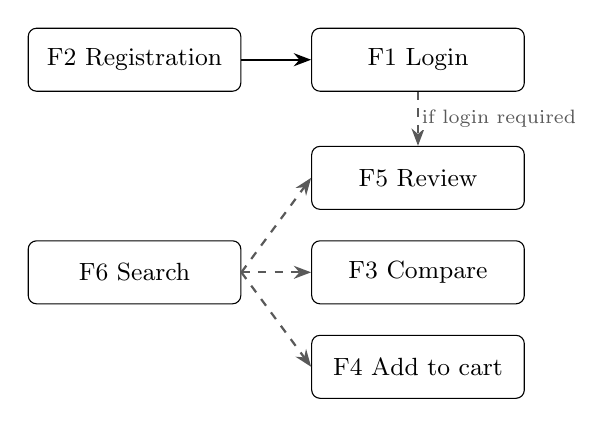
\begin{tikzpicture}[
  fn/.style={draw, rounded corners=3pt, minimum width=2.7cm, minimum height=0.8cm, align=center, font=\small},
  hard/.style={-{Stealth[length=2.2mm]}, thick},
  soft/.style={-{Stealth[length=2.2mm]}, thick, dashed, gray!70!black},
  lab/.style={font=\scriptsize, fill=white, inner sep=1pt}]
  \node[fn] (F2) at (0,0)      {F2 Registration};
  \node[fn] (F1) at (3.6,0)    {F1 Login};
  \node[fn] (F6) at (0,-2.7)   {F6 Search};
  \node[fn] (F5) at (3.6,-1.5) {F5 Review};
  \node[fn] (F3) at (3.6,-2.7) {F3 Compare};
  \node[fn] (F4) at (3.6,-3.9) {F4 Add to cart};
  \draw[hard] (F2) -- (F1);
  \draw[soft] (F6.east) -- (F3.west);
  \draw[soft] (F6.east) -- (F5.west);
  \draw[soft] (F6.east) -- (F4.west);
  \draw[soft] (F1) -- node[lab, right]{if login required} (F5);
\end{tikzpicture}

{\small Solid arrows: hard dependencies. Dashed arrows: test-flow or conditional dependencies.}
\end{center}

%====================================================================
\section*{3. Test Team}
%====================================================================
\instr{Provide the full names, email addresses, subject and tutorial codes of all your team members.}
\instr{Describe the roles and responsibilities of your group members. Make sure that all functions listed in Section 2 are covered.}
\instr{The table below shows an example for your reference.}

Subject: \FILL{31282 or 32571}. Tutorial: \FILL{tutorial code}.

{\renewcommand{\arraystretch}{1.3}
\begin{longtable}{|M{1.9cm}|M{4.1cm}|M{2.9cm}|M{6.6cm}|}
\hline
\bluehead{Student ID} & \bluehead{Member Name} & \bluehead{Role} & \bluehead{Responsibilities (in terms of Function IDs/Names)} \\ \hline
\endhead
26037299 & Nguyen Tran (\href{mailto:nguyenphuongduy.tran@student.uts.edu.au}{\nolinkurl{nguyenphuongduy.tran@student.uts.edu.au}}) & \FILL{e.g. Automation Lead} &
\begin{minipage}[t]{\linewidth}\begin{itemize}[nosep,leftmargin=1.2em]
  \item F6 Searching for a Product
  \item F1 User Login
  \item F5 Submitting a Product Review
\end{itemize}\vspace{2pt}\end{minipage} \\ \hline
\FILL{SID} & \FILL{your name} (\FILL{UTS email}) & \FILL{e.g. Test Lead} &
\begin{minipage}[t]{\linewidth}\begin{itemize}[nosep,leftmargin=1.2em]
  \item F2 User Registration
  \item F3 Comparing Products
  \item F4 Adding a Product to Shopping Cart
\end{itemize}\vspace{2pt}\end{minipage} \\ \hline
\end{longtable}}

Each of the two members tests three functions, so every function in Section 2 has exactly one owner, the workload is balanced, and no two members test the same function:

\begin{center}
{\renewcommand{\arraystretch}{1.2}
\begin{tabular}{|l|c|c|}
\hline
\cellcolor{headgray}\textbf{Function} & \cellcolor{headgray}\textbf{Nguyen Tran} & \cellcolor{headgray}\textbf{\FILL{your name}} \\ \hline
F1 User Login            & \checkmark &  \\ \hline
F2 User Registration     &  & \checkmark \\ \hline
F3 Comparing Products    &  & \checkmark \\ \hline
F4 Add to Cart           &  & \checkmark \\ \hline
F5 Product Review        & \checkmark &  \\ \hline
F6 Search                & \checkmark &  \\ \hline
\end{tabular}}
\end{center}

\vspace{-1ex}
\instr{Indicate whether your group has already delivered (or wishes to deliver) an in-class presentation or submit a recorded presentation.}
{\color{utsblue}\itshape
\begin{itemize}[topsep=0pt]
  \item For an in-class presentation, please indicate which tutorial your group attended (or wishes to attend).
  \item For a recorded presentation, please provide a web link through which your marker can access the recording.
\end{itemize}}

We have not delivered an in-class presentation. \FILL{say whether you wish to present in the Week 12 tutorial (which one), or will not present}

%====================================================================
\section*{4. Task Schedule}
%====================================================================
\instr{Describe the order in which you will test the functions selected in Section 2, either for the whole group or for each member separately. Each function to be tested is considered a \textbf{testing task}. The schedule should be presented using a Gantt chart.}
\instr{Does the order of your testing tasks support parallel testing among team members? If so, explain how. If not, explain how you could improve the schedule to allow members to conduct their testing tasks in parallel.}
\instr{Make sure that you test a function before proceeding to test any function that depends on it. For example, you need to test the ``User Registration'' function first and make sure that it is working before you can test the ``User Login'' function.}
\instr{Make sure to cover all team members (see Section 3) and all functions (see Section 2).}

All six testing tasks finish by 26 October 2026: the two members test in parallel from 21 October, and each member's order respects every dependency in Section 2. Submission is planned for 31 October, one day before the deadline. \FILL{adjust dates to your real plan}

\begin{center}
{\renewcommand{\arraystretch}{1.25}
\begin{tabular}{|l|L{5.6cm}|L{5.6cm}|}
\hline
\cellcolor{headgray}\textbf{Days} & \cellcolor{headgray}\textbf{Nguyen Tran} & \cellcolor{headgray}\textbf{\FILL{your name}} \\ \hline
19--20 Oct & Environment setup & Environment setup \\ \hline
21--22 Oct & F6 Search (no dependencies) & F2 User Registration (no dependencies) \\ \hline
23--24 Oct & F1 User Login (needs F2) & F3 Comparing Products (needs F6) \\ \hline
25--26 Oct & F5 Product Review (needs F6; F1 if login required) & F4 Add to Cart (needs F6) \\ \hline
27--28 Oct & \multicolumn{2}{c|}{Retest failures and log defects (both members)} \\ \hline
29--30 Oct & \multicolumn{2}{c|}{Report integration and review (both members)} \\ \hline
\end{tabular}}
\end{center}

\begin{center}
\resizebox{\textwidth}{!}{%
\begin{ganttchart}[
    time slot format=isodate,
    x unit=0.8cm, y unit chart=0.62cm,
    hgrid, vgrid={*1{draw=black!12}},
    title/.append style={fill=headgray, draw=black!40},
    title label font=\footnotesize,
    bar label font=\small,
    bar/.append style={fill=gray!45, draw=black!50},
    bar height=0.55,
    milestone/.append style={fill=red!70},
    milestone label font=\small\bfseries,
    link/.style={-{Stealth[length=1.6mm]}, thick, black!60}
  ]{2026-10-19}{2026-10-31}
  \gantttitle{October 2026}{13} \\
  \gantttitlecalendar{day} \\
  \ganttbar{Environment setup (both)}{2026-10-19}{2026-10-20} \\
  \ganttbar[name=f6, bar/.append style={fill=memA}]{Nguyen: F6 Search}{2026-10-21}{2026-10-22} \\
  \ganttbar[name=f1, bar/.append style={fill=memA}]{Nguyen: F1 Login}{2026-10-23}{2026-10-24} \\
  \ganttbar[name=f5, bar/.append style={fill=memA}]{Nguyen: F5 Review}{2026-10-25}{2026-10-26} \\
  \ganttbar[name=f2, bar/.append style={fill=memB}]{You: F2 Registration}{2026-10-21}{2026-10-22} \\
  \ganttbar[name=f3, bar/.append style={fill=memB}]{You: F3 Compare}{2026-10-23}{2026-10-24} \\
  \ganttbar[name=f4, bar/.append style={fill=memB}]{You: F4 Add to cart}{2026-10-25}{2026-10-26} \\
  \ganttbar{Retest and defect log (both)}{2026-10-27}{2026-10-28} \\
  \ganttbar{Report integration (both)}{2026-10-29}{2026-10-30} \\
  \ganttmilestone{Submit on Canvas}{2026-10-31}
  \ganttlink{f2}{f1} \ganttlink{f1}{f5}
  \ganttlink{f6}{f3} \ganttlink{f6}{f4}
\end{ganttchart}}

{\small Blue: Nguyen Tran; green: \FILL{your name}. \FILL{replace ``You'' in the bar labels with your name.} Arrows mark dependencies.}
\end{center}

\textbf{Parallel testing.} Yes, the order supports parallel testing. Both members start with a function that depends on nothing (F6 Search and F2 User Registration) and test them at the same time on 21--22 October. Every dependency that crosses between members is therefore already satisfied before it is needed:
\begin{itemize}
  \item F2 (\FILL{your name}) $\rightarrow$ F1 (Nguyen Tran): registration is finished on 22 October, before login testing starts on 23 October.
  \item F6 (Nguyen Tran) $\rightarrow$ F3, F4 (\FILL{your name}): search is finished on 22 October, before comparison and cart testing start.
\end{itemize}
The remaining dependencies (F6 and, if reviews need login, F1 before F5) stay within Nguyen Tran's own queue, so neither member waits for the other at any point.

\textbf{Bottleneck.} F6 gates three functions (F3, F4 and F5). If search fails, the testers open the product page by its direct URL and log the search failure as a defect, so their own testing is not blocked. Each tester also creates their own unique accounts and test data, so parallel runs against the shared live site do not interfere.

%====================================================================
\section*{5. Test Environments and Tools}
%====================================================================
\instr{Describe your computing platforms (Arm, x86), operating systems (macOS, Linux, Windows), and how you set up your testing environments (programming languages, test automation tools, libraries, code editors, and IDEs), step by step.}
\instr{If your group members use different environment configurations or tools, describe each member's environment and tools separately.}

Both members automate with the same stack (Python, pytest and Selenium WebDriver driving Google Chrome) from one shared code repository, so results are comparable; only hardware and operating system differ. The values below were printed on each machine by \texttt{python check\_env.py}.

\begin{center}
{\renewcommand{\arraystretch}{1.25}
\begin{tabular}{|l|L{6.1cm}|L{6.1cm}|}
\hline
\cellcolor{headgray}\textbf{Item} & \cellcolor{headgray}\textbf{Nguyen Tran} & \cellcolor{headgray}\textbf{\FILL{your name}} \\ \hline
Device            & \FILL{e.g. laptop model} & \FILL{} \\ \hline
CPU architecture  & \FILL{x86-64 or Arm64} & \FILL{} \\ \hline
Operating system  & \FILL{e.g. Windows 11 23H2} & \FILL{} \\ \hline
Browser           & Google Chrome \FILL{version} & Google Chrome \FILL{version} \\ \hline
Language          & Python \FILL{version} & Python \FILL{version} \\ \hline
Test framework    & pytest \FILL{version}, pytest-html & pytest \FILL{version}, pytest-html \\ \hline
Automation tool   & Selenium WebDriver \FILL{version}; ChromeDriver via Selenium Manager & Selenium WebDriver \FILL{version}; ChromeDriver via Selenium Manager \\ \hline
IDE / editor      & \FILL{e.g. VS Code + Python extension} & \FILL{} \\ \hline
\end{tabular}}
\end{center}

Setup, step by step (Windows commands; macOS/Linux use \texttt{python3} and \texttt{source .venv/bin/activate}):
\begin{enumerate}[leftmargin=2em, itemsep=1pt]
  \item Install Python 3.9 or later from \url{https://www.python.org/downloads/} (tick ``Add python.exe to PATH'') and Google Chrome; check with \texttt{python --version}.
  \item Install Visual Studio Code and its Python extension.
  \item Download the test suite folder \FILL{GitHub URL} and open PowerShell inside it.
  \item Create and activate a virtual environment: \texttt{python -m venv .venv}, then \texttt{.venv\textbackslash Scripts\textbackslash Activate.ps1}.
  \item Install the libraries: \texttt{python -m pip install -r requirements.txt} (Selenium, pytest, pytest-html). Selenium Manager downloads a ChromeDriver matching the installed Chrome, so no manual driver install is needed.
  \item Record the environment with \texttt{python check\_env.py} (OS, CPU architecture, Python, Selenium, pytest, Chrome and ChromeDriver versions).
  \item Run a test case, e.g.\ \texttt{pytest tests/test\_tc06\_search.py}, or the whole suite with an HTML report: \texttt{pytest --html=report.html --self-contained-html}. Screenshots are saved to \texttt{evidence/}.
\end{enumerate}

%====================================================================
\section*{6. Test Cases}
%====================================================================
\instr{Each group member should complete three test cases -- each corresponding to a function to be tested (in Section 2).}
\instr{The table below shows a sample template for a test case. You need one table for each test case.}
\instr{If your tests have any source code, please provide the source code; if you used any prompts, describe them as well.}
\instr{Examples of test scenarios and steps can be found on page 20 or page 25 of the Tutorial 9 slides, or in feature files (if you use the Gherkin language; see, for example, page 10 of the Tutorial 10 slides).}

Each test case covers one function with three scenarios: a valid path, invalid inputs (input partitioning into equivalence classes), and boundary or edge values (boundary value robustness testing). Every scenario is automated in Python with pytest and Selenium WebDriver; the source file is named in each test case, a screenshot of that code is attached under it, and the full source is in the Appendix.

% ---------------- Test case 1 ----------------
{\renewcommand{\arraystretch}{1.4}
\begin{longtable}{|M{2.6cm}|p{13.6cm}|}
\hline
\bluehead{Test Case ID} & TC01 \\ \hline
\bluehead{Function IDs/Names} & F1 User Login \\ \hline
\bluehead{Tester} & Nguyen Tran \\ \hline
\bluehead{Purpose} & Verify that a registered user can log in with valid credentials, that invalid credentials are rejected with a warning, and that email case is ignored while password case is enforced. \\ \hline
\bluehead{Preconditions} & An account exists, created through F2 in the same run (email \texttt{a3tester.<timestamp>@example.com}, password \texttt{Test@1234}). The browser starts logged out. \\ \hline
\bluehead{Source code} & \texttt{tests/test\_tc01\_login.py} \\ \hline
\scenario{1}{Valid login (success)}{%
  1 & Open \url{https://ecommerce-playground.lambdatest.io/index.php?route=account/login} \\ \hline
  2 & In ``E-Mail Address'', type the registered email. \\ \hline
  3 & In ``Password'', type \texttt{Test@1234}. \\ \hline
  4 & Click \textbf{Login}. \\ \hline
  5 & Check the URL contains \texttt{route=account/account} and the heading is ``My Account''. \\ \hline
  6 & Check the \textbf{Logout} link is offered. Save screenshot \ev{TC01_S1}. \\ \hline
}{The user is logged in and taken to My Account.}
\scenario{2}{Invalid credentials (validation)}{%
  1 & Open the login URL. \\ \hline
  2 & Input (a): registered email + wrong password \texttt{WrongPass99!}; click \textbf{Login}. \\ \hline
  3 & Input (b): unregistered email \texttt{nobody.a3.9z@example.com} + \texttt{Test@1234}; click \textbf{Login}. \\ \hline
  4 & Input (c): both fields left blank; click \textbf{Login}. \\ \hline
  5 & After each input, check the page stays on \texttt{route=account/login} with the warning. Save \ev{TC01_S2a}, \ev{TC01_S2b}, \ev{TC01_S2c}. \\ \hline
}{Each input shows ``Warning: No match for E-Mail Address and/or Password.'' and no session is created.}
\scenario{3}{Letter case of credentials (edge)}{%
  1 & Open the login URL. \\ \hline
  2 & Input (a): registered email in UPPER CASE + \texttt{Test@1234}; click \textbf{Login}; check My Account opens; log out. \\ \hline
  3 & Input (b): registered email + \texttt{TEST@1234} (password case changed); click \textbf{Login}. \\ \hline
  4 & Check (b) stays on the login page with the warning. Save \ev{TC01_S3a}, \ev{TC01_S3b}. \\ \hline
}{(a) succeeds, because email addresses are case-insensitive; (b) is rejected, because passwords are case-sensitive.}
\results{%
  S1  & Valid email + \texttt{Test@1234} & My Account page & \FILL{} & \FILL{} & \ev{TC01_S1} \\ \hline
  S2a & Wrong password & Warning, stays on login & \FILL{} & \FILL{} & \ev{TC01_S2a} \\ \hline
  S2b & Unregistered email & Warning, stays on login & \FILL{} & \FILL{} & \ev{TC01_S2b} \\ \hline
  S2c & Both blank & Warning, stays on login & \FILL{} & \FILL{} & \ev{TC01_S2c} \\ \hline
  S3a & Email upper case & My Account page & \FILL{} & \FILL{} & \ev{TC01_S3a} \\ \hline
  S3b & Password case changed & Warning, stays on login & \FILL{} & \FILL{} & \ev{TC01_S3b} \\ \hline
}
\bluehead{Screenshots} & \shotbox{TC01 evidence and code screenshots}
% \includegraphics[width=\linewidth]{TC01_S1.png}
% \includegraphics[width=\linewidth]{tc01_code.png}
\\ \hline
\end{longtable}}

% ---------------- Test case 2 ----------------
{\renewcommand{\arraystretch}{1.4}
\begin{longtable}{|M{2.6cm}|p{13.6cm}|}
\hline
\bluehead{Test Case ID} & TC02 \\ \hline
\bluehead{Function IDs/Names} & F2 User Registration \\ \hline
\bluehead{Tester} & \FILL{your name} \\ \hline
\bluehead{Purpose} & Verify that a new visitor can register with valid details, that duplicate or invalid submissions are rejected with field-level messages, and that the length limits on First Name (1--32 characters) and Password (4--20 characters) are enforced at their boundaries \VERIFY{limits}. \\ \hline
\bluehead{Preconditions} & Browser logged out. A unique email is generated for each run: \texttt{a3tester.<timestamp>@example.com}. \\ \hline
\bluehead{Source code} & \texttt{tests/test\_tc02\_registration.py} \\ \hline
\scenario{1}{Valid registration (success)}{%
  1 & Open \url{https://ecommerce-playground.lambdatest.io/index.php?route=account/register} \\ \hline
  2 & Enter First Name \texttt{Nam}, Last Name \texttt{Tester}, a unique E-Mail, Telephone \texttt{0412345678}. \\ \hline
  3 & Enter Password \texttt{Test@1234} and Password Confirm \texttt{Test@1234}. \\ \hline
  4 & Leave Newsletter on \textbf{No}; tick \textbf{I have read and agree to the Privacy Policy}. \\ \hline
  5 & Click \textbf{Continue}. \\ \hline
  6 & Check the URL contains \texttt{route=account/success} and the heading ``Your Account Has Been Created!''. Save \ev{TC02_S1}. \\ \hline
}{The account is created and the user is logged in.}
\scenario{2}{Invalid submissions (validation)}{%
  1 & Open the register URL. \\ \hline
  2 & Input (a): all fields valid, but E-Mail = an address already registered; agree; click \textbf{Continue}. \\ \hline
  3 & Input (b): all fields valid with a new email, Privacy Policy \textbf{not} ticked; click \textbf{Continue}. \\ \hline
  4 & Input (c): all fields valid, Password Confirm \texttt{Test@9999}; agree; click \textbf{Continue}. \\ \hline
  5 & After each input, check no account is created and the message appears. Save \ev{TC02_S2a}, \ev{TC02_S2b}, \ev{TC02_S2c}. \\ \hline
}{(a) ``Warning: E-Mail Address is already registered!''; (b) ``Warning: You must agree to the Privacy Policy!''; (c) ``Password confirmation does not match password!''.}
\scenario{3}{Length boundaries (edge)}{%
  1 & Open the register URL. \\ \hline
  2 & Input (a): First Name of 33 characters (\texttt{A} $\times$ 33), other fields valid; agree; click \textbf{Continue}. \\ \hline
  3 & Input (b): Password and Confirm of 3 characters \texttt{Ab1}, other fields valid; agree; click \textbf{Continue}. \\ \hline
  4 & Input (c): First Name of exactly 32 characters, Password and Confirm of exactly 4 characters \texttt{Ab1!}, new email; agree; click \textbf{Continue}. \\ \hline
  5 & Save \ev{TC02_S3a}, \ev{TC02_S3b}, \ev{TC02_S3c}. \\ \hline
}{(a) ``First Name must be between 1 and 32 characters!''; (b) ``Password must be between 4 and 20 characters!''; (c) the account is created, because 32 and 4 are inside the limits.}
\results{%
  S1  & All fields valid & Account created & \FILL{} & \FILL{} & \ev{TC02_S1} \\ \hline
  S2a & Duplicate email & Already-registered warning & \FILL{} & \FILL{} & \ev{TC02_S2a} \\ \hline
  S2b & Policy not ticked & Privacy Policy warning & \FILL{} & \FILL{} & \ev{TC02_S2b} \\ \hline
  S2c & Confirm mismatch & Mismatch message & \FILL{} & \FILL{} & \ev{TC02_S2c} \\ \hline
  S3a & First Name 33 chars & Length message & \FILL{} & \FILL{} & \ev{TC02_S3a} \\ \hline
  S3b & Password 3 chars & Length message & \FILL{} & \FILL{} & \ev{TC02_S3b} \\ \hline
  S3c & Name 32, password 4 & Account created & \FILL{} & \FILL{} & \ev{TC02_S3c} \\ \hline
}
\bluehead{Screenshots} & \shotbox{TC02 evidence and code screenshots}
% \includegraphics[width=\linewidth]{TC02_S1.png}
\\ \hline
\end{longtable}}

% ---------------- Test case 3 ----------------
{\renewcommand{\arraystretch}{1.4}
\begin{longtable}{|M{2.6cm}|p{13.6cm}|}
\hline
\bluehead{Test Case ID} & TC03 \\ \hline
\bluehead{Function IDs/Names} & F3 Comparing Products \\ \hline
\bluehead{Tester} & \FILL{your name} \\ \hline
\bluehead{Purpose} & Verify that products added to the comparison list appear side by side with correct details, that products can be removed until the list is empty, and that the list keeps at most four products. \\ \hline
\bluehead{Preconditions} & F6 Search works. New browser session, so the comparison list starts empty. Products (product\_id): iPod Touch 32, iPod Nano 36, iPod Shuffle 34, iPod Classic 48, iPhone 40. \\ \hline
\bluehead{Source code} & \texttt{tests/test\_tc03\_compare.py} \\ \hline
\scenario{1}{Compare two products (success)}{%
  1 & Open the home page and search \texttt{iPod} (F6). \\ \hline
  2 & Open \textbf{iPod Touch}; click \textbf{Compare this Product}. \\ \hline
  3 & Check the alert ``Success: You have added iPod Touch to your product comparison!''. \\ \hline
  4 & Return to the results; open \textbf{iPod Nano}; click \textbf{Compare this Product}. \\ \hline
  5 & Open \url{https://ecommerce-playground.lambdatest.io/index.php?route=product/compare} \\ \hline
  6 & Check both products are columns of the table, each with name, price, model and availability matching its product page. Save \ev{TC03_S1}. \\ \hline
}{A two-column comparison with correct details for both products.}
\scenario{2}{Remove products and empty list (validation)}{%
  1 & Continue from Scenario 1 on the comparison page. \\ \hline
  2 & Click \textbf{Remove} under iPod Touch. \\ \hline
  3 & Check ``Success: You have modified your product comparison!'' and that only iPod Nano remains. Save \ev{TC03_S2a}. \\ \hline
  4 & Click \textbf{Remove} under iPod Nano; check ``You have not chosen any products to compare.''. Save \ev{TC03_S2b}. \\ \hline
  5 & Open the comparison URL in a fresh session; check the same empty message and no error page. Save \ev{TC03_S2c}. \\ \hline
}{Each removal updates the table; an empty list shows the empty message, not an error.}
\scenario{3}{List size limit and duplicates (edge)}{%
  1 & In a fresh session add, in order: iPod Touch, iPod Nano, iPod Shuffle, iPod Classic (4 products). \\ \hline
  2 & Open the comparison page; check 4 columns. Save \ev{TC03_S3a}. \\ \hline
  3 & Add a fifth product, iPhone; open the comparison page. Save \ev{TC03_S3b}. \\ \hline
  4 & Add iPhone a second time; open the comparison page. Save \ev{TC03_S3c}. \\ \hline
}{(a) 4 columns; (b) still 4 columns, iPhone added and the oldest product (iPod Touch) dropped; (c) iPhone appears once only.}
\results{%
  S1  & Add 2 products & 2 columns, details correct & \FILL{} & \FILL{} & \ev{TC03_S1} \\ \hline
  S2a & Remove 1 of 2 & 1 column left & \FILL{} & \FILL{} & \ev{TC03_S2a} \\ \hline
  S2b & Remove last & Empty-list message & \FILL{} & \FILL{} & \ev{TC03_S2b} \\ \hline
  S2c & Empty list by URL & Empty-list message & \FILL{} & \FILL{} & \ev{TC03_S2c} \\ \hline
  S3a & 4 products & 4 columns & \FILL{} & \FILL{} & \ev{TC03_S3a} \\ \hline
  S3b & 5th product & 4 columns, oldest dropped & \FILL{} & \FILL{} & \ev{TC03_S3b} \\ \hline
  S3c & Same product twice & Listed once & \FILL{} & \FILL{} & \ev{TC03_S3c} \\ \hline
}
\bluehead{Screenshots} & \shotbox{TC03 evidence and code screenshots}
% \includegraphics[width=\linewidth]{TC03_S1.png}
\\ \hline
\end{longtable}}

% ---------------- Test case 4 ----------------
{\renewcommand{\arraystretch}{1.4}
\begin{longtable}{|M{2.6cm}|p{13.6cm}|}
\hline
\bluehead{Test Case ID} & TC04 \\ \hline
\bluehead{Function IDs/Names} & F4 Adding a Product to Shopping Cart \\ \hline
\bluehead{Tester} & \FILL{your name} \\ \hline
\bluehead{Purpose} & Verify that valid quantities are added and totalled correctly, that zero, negative and non-numeric quantities are rejected, and how the cart handles a quantity above available stock. \\ \hline
\bluehead{Preconditions} & F6 Search works. New browser session with an empty cart. Product: iPod Touch (\texttt{product\_id=32}), listed at \$194.00 on 17 October 2026 and in stock \VERIFY{price and stock on the day}. \\ \hline
\bluehead{Source code} & \texttt{tests/test\_tc04\_add\_to\_cart.py} \\ \hline
\scenario{1}{Add valid quantities (success)}{%
  1 & Search \texttt{iPod Touch} (F6) and open \url{https://ecommerce-playground.lambdatest.io/index.php?route=product/product&product_id=32} \\ \hline
  2 & Note the unit price. Leave Qty = \texttt{1}; click \textbf{Add to Cart}. \\ \hline
  3 & Check the alert ``Success: You have added iPod Touch to your shopping cart!'' and the header cart count = 1. Save \ev{TC04_S1a}. \\ \hline
  4 & Set Qty = \texttt{2}; click \textbf{Add to Cart} again. \\ \hline
  5 & Open \url{https://ecommerce-playground.lambdatest.io/index.php?route=checkout/cart} \\ \hline
  6 & Check one iPod Touch line with quantity 3 and the line total below. Save \ev{TC04_S1b}. \\ \hline
}{One cart line of 3 $\times$ iPod Touch. The expected line total is three times the unit price noted in step 2:
\[ \text{Line total} = 3 \times \$194.00 = \$582.00 \]}
\scenario{2}{Invalid quantities (validation)}{%
  1 & Start a fresh session (empty cart) and open the iPod Touch product page. \\ \hline
  2 & Input (a): Qty = \texttt{0}; click \textbf{Add to Cart}; record the message and cart count. Save \ev{TC04_S2a}. \\ \hline
  3 & Input (b): Qty = \texttt{-1}; click \textbf{Add to Cart}; record the message and count. Save \ev{TC04_S2b}. \\ \hline
  4 & Input (c): Qty = \texttt{abc}; click \textbf{Add to Cart}; record the message and count. Save \ev{TC04_S2c}. \\ \hline
  5 & Open the cart page; check it is still empty. \\ \hline
}{Each invalid quantity is rejected (a minimum-quantity warning, or the field refuses the value) and the cart stays empty.}
\scenario{3}{Quantity above stock (edge)}{%
  1 & Start a fresh session and open the iPod Touch product page. \\ \hline
  2 & Set Qty = \texttt{9999}; click \textbf{Add to Cart}. \\ \hline
  3 & Open the cart page. Save \ev{TC04_S3a}. \\ \hline
  4 & Click \textbf{Checkout}. Save \ev{TC04_S3b}. \\ \hline
}{The cart marks the line with *** and shows ``Products marked with *** are not available in the desired quantity or not in stock!''; checkout does not proceed for that quantity \VERIFY{store stock setting}.}
\results{%
  S1a & Qty 1 & Success alert, count 1 & \FILL{} & \FILL{} & \ev{TC04_S1a} \\ \hline
  S1b & Qty 2 more & 1 line, qty 3, total $3\times$ unit price & \FILL{} & \FILL{} & \ev{TC04_S1b} \\ \hline
  S2a & Qty 0 & Rejected, cart empty & \FILL{} & \FILL{} & \ev{TC04_S2a} \\ \hline
  S2b & Qty $-1$ & Rejected, cart empty & \FILL{} & \FILL{} & \ev{TC04_S2b} \\ \hline
  S2c & Qty \texttt{abc} & Rejected, cart empty & \FILL{} & \FILL{} & \ev{TC04_S2c} \\ \hline
  S3a & Qty 9999 & Stock warning in cart & \FILL{} & \FILL{} & \ev{TC04_S3a} \\ \hline
  S3b & Checkout with 9999 & Order blocked & \FILL{} & \FILL{} & \ev{TC04_S3b} \\ \hline
}
\bluehead{Screenshots} & \shotbox{TC04 evidence and code screenshots}
% \includegraphics[width=\linewidth]{TC04_S1b.png}
\\ \hline
\end{longtable}}

% ---------------- Test case 5 ----------------
{\renewcommand{\arraystretch}{1.4}
\begin{longtable}{|M{2.6cm}|p{13.6cm}|}
\hline
\bluehead{Test Case ID} & TC05 \\ \hline
\bluehead{Function IDs/Names} & F5 Submitting a Product Review \\ \hline
\bluehead{Tester} & Nguyen Tran \\ \hline
\bluehead{Purpose} & Verify that a complete review is accepted for moderation, that missing or out-of-range fields are rejected with the right warning, and that the review-text limits (25--1000 characters) are enforced exactly at their boundaries \VERIFY{limits}. \\ \hline
\bluehead{Preconditions} & F6 Search works. Review form open on the iPod Touch page (\texttt{product\_id=32}). If the form asks guests to log in, log in first with the TC01 account (F1) \VERIFY{guest reviews}. \\ \hline
\bluehead{Source code} & \texttt{tests/test\_tc05\_review.py} \\ \hline
\scenario{1}{Valid review (success)}{%
  1 & Search \texttt{iPod Touch} (F6), open the product page and the \textbf{Write a review} form. \\ \hline
  2 & Your Name: \texttt{Nam T}. \\ \hline
  3 & Your Review: ``Great sound quality and the battery easily lasts a full day of use.'' (67 characters). \\ \hline
  4 & Rating: 4 stars. \\ \hline
  5 & Click \textbf{Write Review}. \\ \hline
  6 & Check the success message. Save \ev{TC05_S1}. \\ \hline
}{``Thank you for your review. It has been submitted to the webmaster for approval.'' The review is not public until an administrator approves it (out of scope).}
\scenario{2}{Missing or invalid fields (validation)}{%
  1 & Reload the product page and open the review form for each input. \\ \hline
  2 & Input (a): Name \texttt{Nam T}, valid 67-character text, \textbf{no rating}; submit. Save \ev{TC05_S2a}. \\ \hline
  3 & Input (b): Name \texttt{Na} (2 characters), valid text, rating 4; submit. Save \ev{TC05_S2b}. \\ \hline
  4 & Input (c): Name \texttt{Nam T}, text ``Too short.'' (10 characters), rating 4; submit. Save \ev{TC05_S2c}. \\ \hline
}{(a) ``Warning: Please select a review rating!''; (b) ``Warning: Review Name must be between 3 and 25 characters!''; (c) ``Warning: Review Text must be between 25 and 1000 characters!''. No review is submitted.}
\scenario{3}{Review-text boundaries (edge)}{%
  1 & Reload the product page for each input; Name \texttt{Nam T}, rating 5. \\ \hline
  2 & Input (a): text of exactly 24 characters; submit. \\ \hline
  3 & Input (b): text of exactly 25 characters; submit. \\ \hline
  4 & Input (c): text of exactly 1000 characters; submit. \\ \hline
  5 & Input (d): text of exactly 1001 characters; submit. Save \ev{TC05_S3a} to \ev{TC05_S3d}. \\ \hline
}{(a) and (d) show the review-text length warning; (b) and (c) show the success message.}
\results{%
  S1  & Valid name, text, 4 stars & Submitted for approval & \FILL{} & \FILL{} & \ev{TC05_S1} \\ \hline
  S2a & No rating & Rating warning & \FILL{} & \FILL{} & \ev{TC05_S2a} \\ \hline
  S2b & Name 2 chars & Name length warning & \FILL{} & \FILL{} & \ev{TC05_S2b} \\ \hline
  S2c & Text 10 chars & Text length warning & \FILL{} & \FILL{} & \ev{TC05_S2c} \\ \hline
  S3a & Text 24 chars & Text length warning & \FILL{} & \FILL{} & \ev{TC05_S3a} \\ \hline
  S3b & Text 25 chars & Submitted & \FILL{} & \FILL{} & \ev{TC05_S3b} \\ \hline
  S3c & Text 1000 chars & Submitted & \FILL{} & \FILL{} & \ev{TC05_S3c} \\ \hline
  S3d & Text 1001 chars & Text length warning & \FILL{} & \FILL{} & \ev{TC05_S3d} \\ \hline
}
\bluehead{Screenshots} & \shotbox{TC05 evidence and code screenshots}
% \includegraphics[width=\linewidth]{TC05_S1.png}
\\ \hline
\end{longtable}}

% ---------------- Test case 6 ----------------
{\renewcommand{\arraystretch}{1.4}
\begin{longtable}{|M{2.6cm}|p{13.6cm}|}
\hline
\bluehead{Test Case ID} & TC06 \\ \hline
\bluehead{Function IDs/Names} & F6 Searching for a Product \\ \hline
\bluehead{Tester} & Nguyen Tran \\ \hline
\bluehead{Purpose} & Verify that matching keywords return relevant products, that unmatched, blank and script-like input is handled safely with a clear message, and that search is not sensitive to letter case, partial words or surrounding spaces. \\ \hline
\bluehead{Preconditions} & Any page of the site is open; no login needed. \\ \hline
\bluehead{Source code} & \texttt{tests/test\_tc06\_search.py} \\ \hline
\scenario{1}{Matching keyword (success)}{%
  1 & Open \url{https://ecommerce-playground.lambdatest.io/index.php?route=common/home} \\ \hline
  2 & Click the header search box and type \texttt{iPod}. \\ \hline
  3 & Press \textbf{Enter}. \\ \hline
  4 & Check the URL contains \texttt{route=product/search\&search=iPod} and the heading ``Search - iPod''. \\ \hline
  5 & Check at least one product is listed and every product name contains ``iPod''. Save \ev{TC06_S1}. \\ \hline
}{A results page listing only iPod products (e.g.\ iPod Touch, iPod Nano, iPod Shuffle, iPod Classic).}
\scenario{2}{Non-matching, blank and script input (validation)}{%
  1 & From the home page, type each input in the search box and press \textbf{Enter}. \\ \hline
  2 & Input (a): \texttt{xyzqwe123} (no such product). Save \ev{TC06_S2a}. \\ \hline
  3 & Input (b): blank search box. Save \ev{TC06_S2b}. \\ \hline
  4 & Input (c): \texttt{<script>alert(1)</script>}; check no browser alert opens and the text is shown as plain text. Save \ev{TC06_S2c}. \\ \hline
}{(a) and (c) show ``There is no product that matches the search criteria.''; (b) shows the search page with no products and no error; (c) never executes the script.}
\scenario{3}{Case, partial word and spaces (edge)}{%
  1 & Search \texttt{iPod} and record the number of results $N$ (baseline). \\ \hline
  2 & Input (a): \texttt{IPOD}; record the count. \\ \hline
  3 & Input (b): \texttt{ipo} (partial word); record the count and check every name contains ``iPod''. \\ \hline
  4 & Input (c): \texttt{\ \ \ iPod\ \ \ } (spaces before and after); record the count. Save \ev{TC06_S3a} to \ev{TC06_S3c}. \\ \hline
}{(a), (b) and (c) each return the same $N$ products as \texttt{iPod}.}
\results{%
  S1  & \texttt{iPod} & iPod products only & \FILL{} & \FILL{} & \ev{TC06_S1} \\ \hline
  S2a & \texttt{xyzqwe123} & No-match message & \FILL{} & \FILL{} & \ev{TC06_S2a} \\ \hline
  S2b & Blank & No products, no error & \FILL{} & \FILL{} & \ev{TC06_S2b} \\ \hline
  S2c & Script tag & No-match message, no alert & \FILL{} & \FILL{} & \ev{TC06_S2c} \\ \hline
  S3a & \texttt{IPOD} & Same $N$ as \texttt{iPod} & \FILL{} & \FILL{} & \ev{TC06_S3a} \\ \hline
  S3b & \texttt{ipo} & Same $N$ as \texttt{iPod} & \FILL{} & \FILL{} & \ev{TC06_S3b} \\ \hline
  S3c & Spaces around \texttt{iPod} & Same $N$ as \texttt{iPod} & \FILL{} & \FILL{} & \ev{TC06_S3c} \\ \hline
}
\bluehead{Screenshots} & \shotbox{TC06 evidence and code screenshots}
% \includegraphics[width=\linewidth]{TC06_S1.png}
\\ \hline
\end{longtable}}


%====================================================================
\section*{7. Analysis and Reflections}
%====================================================================
\instr{Provide basic statistics for the tests conducted by your group, including how many passed, failed, or resulted in errors. List any defects that you identified on the website.}
\instr{Reflect on the tests you have conducted and identify the successes and failures in your group's efforts. What lessons did you learn? How would you approach the system testing tasks differently if given a second chance?}

\textbf{Test statistics.} The group executed \FILL{N} test cases containing \FILL{M} scenario checks: \FILL{x} passed, \FILL{y} failed and \FILL{z} ended in an error. A test case counts as passed only if every one of its checks passed. A \emph{fail} means the site behaved differently from the expected result (a possible defect); an \emph{error} means the test could not complete (for example a locator was not found or the site timed out), which is a problem with the test rather than the site.

\begin{center}
{\renewcommand{\arraystretch}{1.2}
\begin{tabular}{|l|l|c|c|c|c|c|}
\hline
\cellcolor{headgray}\textbf{Test case} & \cellcolor{headgray}\textbf{Function} & \cellcolor{headgray}\textbf{Checks} & \cellcolor{headgray}\textbf{Passed} & \cellcolor{headgray}\textbf{Failed} & \cellcolor{headgray}\textbf{Errors} & \cellcolor{headgray}\textbf{Result} \\ \hline
TC01 & F1 User Login           & 6 & \FILL{} & \FILL{} & \FILL{} & \FILL{} \\ \hline
TC02 & F2 User Registration    & 7 & \FILL{} & \FILL{} & \FILL{} & \FILL{} \\ \hline
TC03 & F3 Comparing Products   & 7 & \FILL{} & \FILL{} & \FILL{} & \FILL{} \\ \hline
TC04 & F4 Add to Cart          & 7 & \FILL{} & \FILL{} & \FILL{} & \FILL{} \\ \hline
TC05 & F5 Product Review       & 8 & \FILL{} & \FILL{} & \FILL{} & \FILL{} \\ \hline
TC06 & F6 Search               & 7 & \FILL{} & \FILL{} & \FILL{} & \FILL{} \\ \hline
\textbf{Total} &               & 42 & \FILL{} & \FILL{} & \FILL{} & \FILL{} \\ \hline
\end{tabular}}
\end{center}

\textbf{Defects found.} Severity: High = blocks a core purchase or account task; Medium = wrong result with a workaround; Low = cosmetic or wording. \FILL{list only defects actually observed; if none, write ``No defects were found in the functions tested.''}

{\small\renewcommand{\arraystretch}{1.25}
\begin{longtable}{|L{0.8cm}|L{1.4cm}|L{2.8cm}|L{1.4cm}|L{3.2cm}|L{2.4cm}|L{2.4cm}|}
\hline
\cellcolor{headgray}\textbf{ID} & \cellcolor{headgray}\textbf{Test} & \cellcolor{headgray}\textbf{Description} & \cellcolor{headgray}\textbf{Severity} & \cellcolor{headgray}\textbf{Steps to reproduce} & \cellcolor{headgray}\textbf{Expected} & \cellcolor{headgray}\textbf{Actual} \\ \hline
D01 & \FILL{} & \FILL{} & \FILL{} & \FILL{} & \FILL{} & \FILL{} \\ \hline
D02 & \FILL{} & \FILL{} & \FILL{} & \FILL{} & \FILL{} & \FILL{} \\ \hline
\end{longtable}}

\textbf{Reflections.} \FILL{edit every sentence to match what really happened}
Ordering the work by function dependencies let both members test in parallel from the first testing day: each started with a function that depends on nothing (registration and search), so every cross-member prerequisite was already done when it was needed. Automating every scenario in pytest and Selenium made re-runs cheap, so failures could be re-checked before being logged as defects. The main technical challenge was locating elements reliably: the site's theme renders duplicate search boxes and buttons for desktop and mobile, so locators had to select the visible element and wait explicitly for alerts. Testing against a shared, public demo site also meant state we did not control, such as stock levels, other users' data and reviews held for moderation, so each tester generated unique accounts and kept expected results independent of existing data. Team coordination worked through one shared repository with common helper code, which kept browser setup, screenshots and test data consistent across members. We learned that boundary values and invalid inputs exposed more issues than the valid paths, and that writing a precise expected result before running a test makes the pass/fail decision objective. Given a second attempt, we would adopt the Page Object Model from the start, run the suite in Chrome and Firefox through Selenium Grid, and add a continuous integration workflow so every change re-runs the tests automatically.

%====================================================================
\clearpage
\section*{Appendix: Test Source Code}
%====================================================================
Repository: \FILL{public GitHub URL}. To print the code here, upload the test suite to Overleaf keeping its folders (\texttt{helpers.py}, \texttt{conftest.py}, \texttt{tests/}); any file not uploaded shows a red note instead of breaking the build.

\subsection*{helpers.py}
\codefile{helpers.py}
\subsection*{conftest.py}
\codefile{conftest.py}
\subsection*{tests/test\_tc01\_login.py}
\codefile{tests/test_tc01_login.py}
\subsection*{tests/test\_tc02\_registration.py}
\codefile{tests/test_tc02_registration.py}
\subsection*{tests/test\_tc03\_compare.py}
\codefile{tests/test_tc03_compare.py}
\subsection*{tests/test\_tc04\_add\_to\_cart.py}
\codefile{tests/test_tc04_add_to_cart.py}
\subsection*{tests/test\_tc05\_review.py}
\codefile{tests/test_tc05_review.py}
\subsection*{tests/test\_tc06\_search.py}
\codefile{tests/test_tc06_search.py}

\end{document}